\documentclass[10pt]{beamer}

\usetheme[progressbar=frametitle, sectionpage=none]{metropolis}
\usepackage{appendixnumberbeamer}
\usepackage{pgfpages}
\usepackage{booktabs}
\usepackage[dvipsnames]{xcolor}
\usepackage{mathtools}

\usepackage{pgfplots}

\usepgfplotslibrary{dateplot}

\setbeameroption{slides only}
%\setbeameroption{show only notes}
%\setbeameroption{show notes on second screen=right}
\usepackage{xspace}
\newcommand{\themename}{\textbf{\textsc{metropolis}}\xspace}

\title{Labor Markets and Technological Change: Evidence from Electronic Health Records}

\subtitle{Hanna Glenn\\ \small Emory University}
 \date{\today}

\setbeamertemplate{caption}{\raggedright\insertcaption\par}
\setbeamertemplate{itemize item}{\scalebox{.6}{$\blacktriangleright$ }}     
\setbeamertemplate{itemize subitem}{\scalebox{.8}{$\centerdot$ }} 

\begin{document}

\maketitle

\setbeamercolor{background canvas}{bg=white}




\section[Motivation]{Motivation}

\begin{frame}{Big Picture}
\begin{itemize}
    \item Longstanding topic in economics: relationship between technology and employment
    \vspace{2mm}
    \begin{itemize}
        \item Displacement?
        \item Productivity?
    \end{itemize}
    \vspace{3mm}
    \item Investigated in many settings
    \vspace{3mm}
    \item The answer depends heavily on the setting
    \vspace{3mm}
    \item This paper: specific healthcare setting
\end{itemize}

\end{frame}

\begin{frame}[fragile]{What is an Electronic Health Record?}
``An electronic health record is the systematized collection of patient and population electronically stored health information in a digital format"

\vspace{3mm}

What it can do:
\begin{itemize}
    \item Paper $\rightarrow$ computerization
    \item Communication
    \item Decision making assistance
\end{itemize}

\end{frame}

\begin{frame}[fragile]{HIT: Great (Expected) Potential in Healthcare}
\begin{alertblock}{Cost Saving}
\begin{itemize}
    \item Possible cost reduction of hundreds of billions of dollars \\ \scriptsize (Hillestad et al 2005)
\end{itemize}
\end{alertblock}

\begin{alertblock}{Quality Improvement}
\begin{itemize}
    \item Improved efficiency, patient safety improvements, physicians have decision support that could prevent unnecessary complications, etc.
\end{itemize}
\end{alertblock}

\vspace{4mm}

Significant policy push for EHR implementation: HITECH Act, 2008 provided financial incentive for hospitals to implement EHRs
\begin{itemize}
    \item \textcolor{blue}{The percentage of hospitals with basic EHR capability rose from 9$\%$ in 2008 to 84$\%$ in 2015.} \scriptsize (Health IT Dashboard)
\end{itemize}

\end{frame}


\begin{frame}{Physician Response to EHRs}
\begin{center}
    
\includegraphics[scale=.3]{graphics/News Clip3.PNG}
    
    \vspace{3mm}
    
    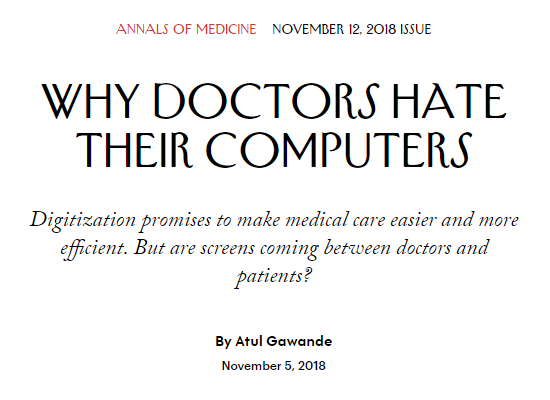
\includegraphics[scale=.3]{graphics/News Clip2.PNG}
\end{center}

\end{frame}


\begin{frame}{This Paper}

Did EHR implementation in hospitals affect physician labor market decisions?
\begin{itemize}
    \item Intensive Margin / Productivity
    \item Extensive Margin / Retirement
    \item Hospital $\rightarrow$ Office
\end{itemize}

\end{frame}


\section{Contribution}

\begin{frame}{Literature}
\small
\begin{columns}
\setlength{\tabcolsep}{-5pt}
    \column{0.4\textwidth}
        \centering
        \underline{ Technology $\rightarrow$ Labor }
        \vspace{-1mm}
        \begin{itemize}
            \item Erosion effect vs. wage effect \\ \vspace{1mm}
            \tiny (Zeira $\&$ Joseph 2011, EJ)
            
            \footnotesize
            
            \item Cause retirement? \\ \vspace{1mm}
            \tiny (Schleife 2006, Labour; Cavapozzi et al 2013, AE; Roger et al 2006, EJ; Friedburg 2003, ILRR)
            
            \footnotesize
            
            \item Older, well educated members of labor force exited at higher rates due to computerization \\ \vspace{1mm}
            \tiny (Willis and Hudomiet 2021, Labour)
            
            \footnotesize 
            
            \item Computerization in white collar jobs leads to decrease in employment for the same jobs that implemented the technology \\ \vspace{1mm}
            \tiny (Dillender & Forsythe 2022, NBER)
        \end{itemize}
        
        
        \column{0.4\textwidth}
        \centering
        
        \pause
        
        \color{blue}
        \underline{ Contribution }
        
        \vspace{1mm}
 
            \begin{itemize}
            \color{blue}
                \item While doctors are white collar, their labor market incentives differ from many other jobs
                \item Population of physicians - possible shortages / access to care issues
            \end{itemize}

        
\end{columns}
\end{frame}



\begin{frame}{Literature}
\small
\begin{columns}
\setlength{\tabcolsep}{-5pt}
        \column{0.4\textwidth}
        \centering
        \underline{ EHR $\rightarrow$ Healthcare }
        \vspace{-1mm}
        \begin{itemize}
            \item Small improvements for severe health conditions \\ \vspace{1mm}
            \tiny(Agha 2014, JHE; McCullough et al 2016, RAND)
            
            \footnotesize
            
            \item No decrease in cost \\ \vspace{1mm}
            \tiny (Agha 2014, JHE; Dranove et al 2019, AEJ) 
            
            \footnotesize
            
            \item Productivity and opinion about EHRs varies drastically \\ \vspace{1mm}
            \tiny (Hitt $\&$ Tambe 2016, ILRR; Butler $\&$ Johnson 2016, IJHEM; Meyerhoefer et al 2016, ILRR)
        \end{itemize}
        
        \pause
        
        \column{0.4\textwidth}
        \centering
        \color{blue}
        \underline{ Contribution }
        \vspace{1mm}
        \begin{itemize}
        \color{blue}
            \item No empirical work on EHR/physician effects
            \item Speaks to the puzzling results
            \item Time period 
        \end{itemize}
        
        
\end{columns}

\end{frame}




\section{Data}

\begin{frame}{Data}
    \underline{CMS Shared Patient Data (2009-2015)}
    \begin{itemize}
        \item Hospital-physician pairs: bill for same patient under Medicare
        \item Physician (PCP, hospitalist, internist) works in the hospital
    \end{itemize}
    
    \vspace{3mm}
    
    \underline{Medicare Data on Provider Practice and Specialty (2009-2017)}
    \begin{itemize}
        \item Physician-level number of unique patients, primary locations of practice, and total claims 
    \end{itemize}
    
    \vspace{3mm}
    
    \underline{EHR Use:}
    \begin{itemize}
        \item AHA Survey Question
    \end{itemize}
    
    \vspace{3mm}
    
    \underline{Physician Compare}: Age of physician
    
    \vspace{3mm}
    
    $\rightarrow$ Final data is at the physician level from 2009-2017, where only physicians who are exposed by 2015 are included 
\end{frame}


\begin{frame}{Variables}

Labor Market Outcomes:
\begin{itemize}
    \item Retirement
    \begin{itemize}
        \item Physicians stop seeing patients $\rightarrow$ drop out of data
    \end{itemize}
    
    \item Work Setting:
    \begin{itemize}
        \item Percentage of patients seen in an office setting
        \item Indicator for seeing any patients in an office setting
        \item Indicator for changing zip codes
    \end{itemize}
    
    \item Productivity:
    \begin{itemize}
        \item Number of patients
        \item Ratio of claims per patient
    \end{itemize}
\end{itemize}

EHR Use:
\vspace{-2mm}
\begin{itemize}
    \item Indicator for any exposure to EHR at related hospitals
\end{itemize}

\end{frame}


\begin{frame}{Data}
    \centering
    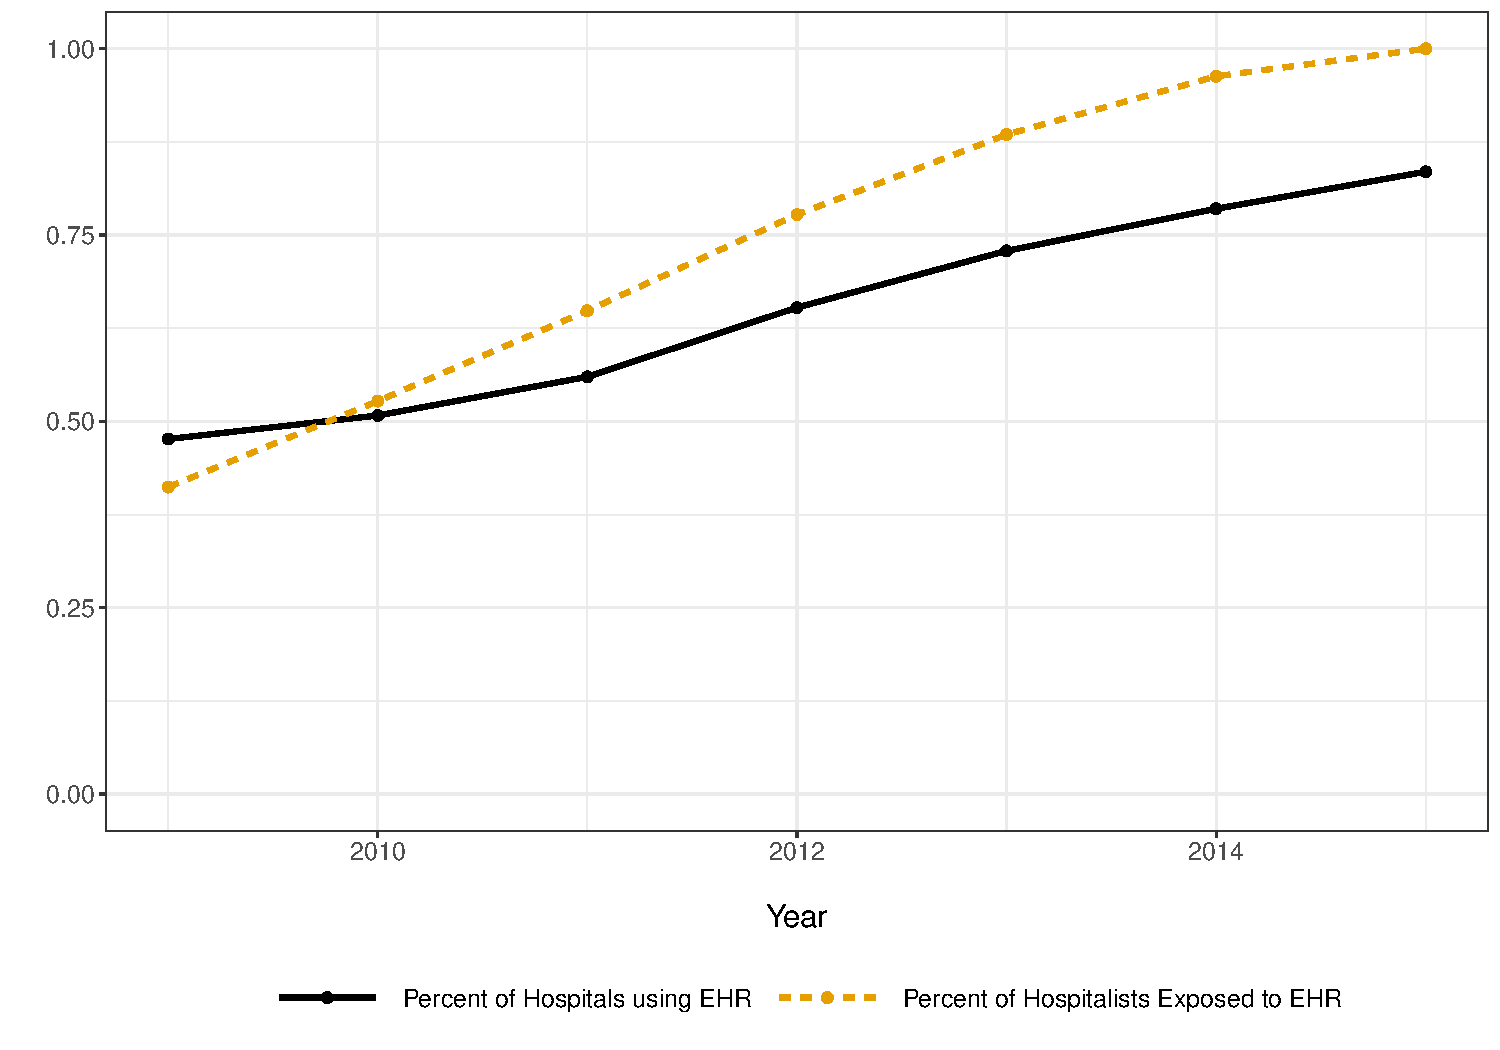
\includegraphics[scale=.4]{Objects/sum_stats_year.pdf}
\end{frame}



\section{Analysis}


\begin{frame}{Event Study}

\begin{itemize}
    \item Since I have differential timing of exposure, I use Callaway and Sant'Anna (2021) average group time treatment effects
    \vspace{3mm}
    $$ATT(g,t)=\mathbbm{E}[Y_t(g)-Y_t(0)|G_g=1]$$
    \vspace{3mm}
    \item Aggregate these over groups to get a familiar event study plot
\end{itemize}
    
\end{frame}

\begin{frame}{Assumptions}
\begin{itemize}
    \item No reversal of treatment
    \item No anticipation of treatment (can be relaxed)
    \item Parallel trends
    \item Institutional assumption: physicians are constrained to use to technology implemented in their hospital
\end{itemize}
    
\end{frame}

\section{Results}


\begin{frame}{Retirement}
\begin{figure}[ht]
    \centering
    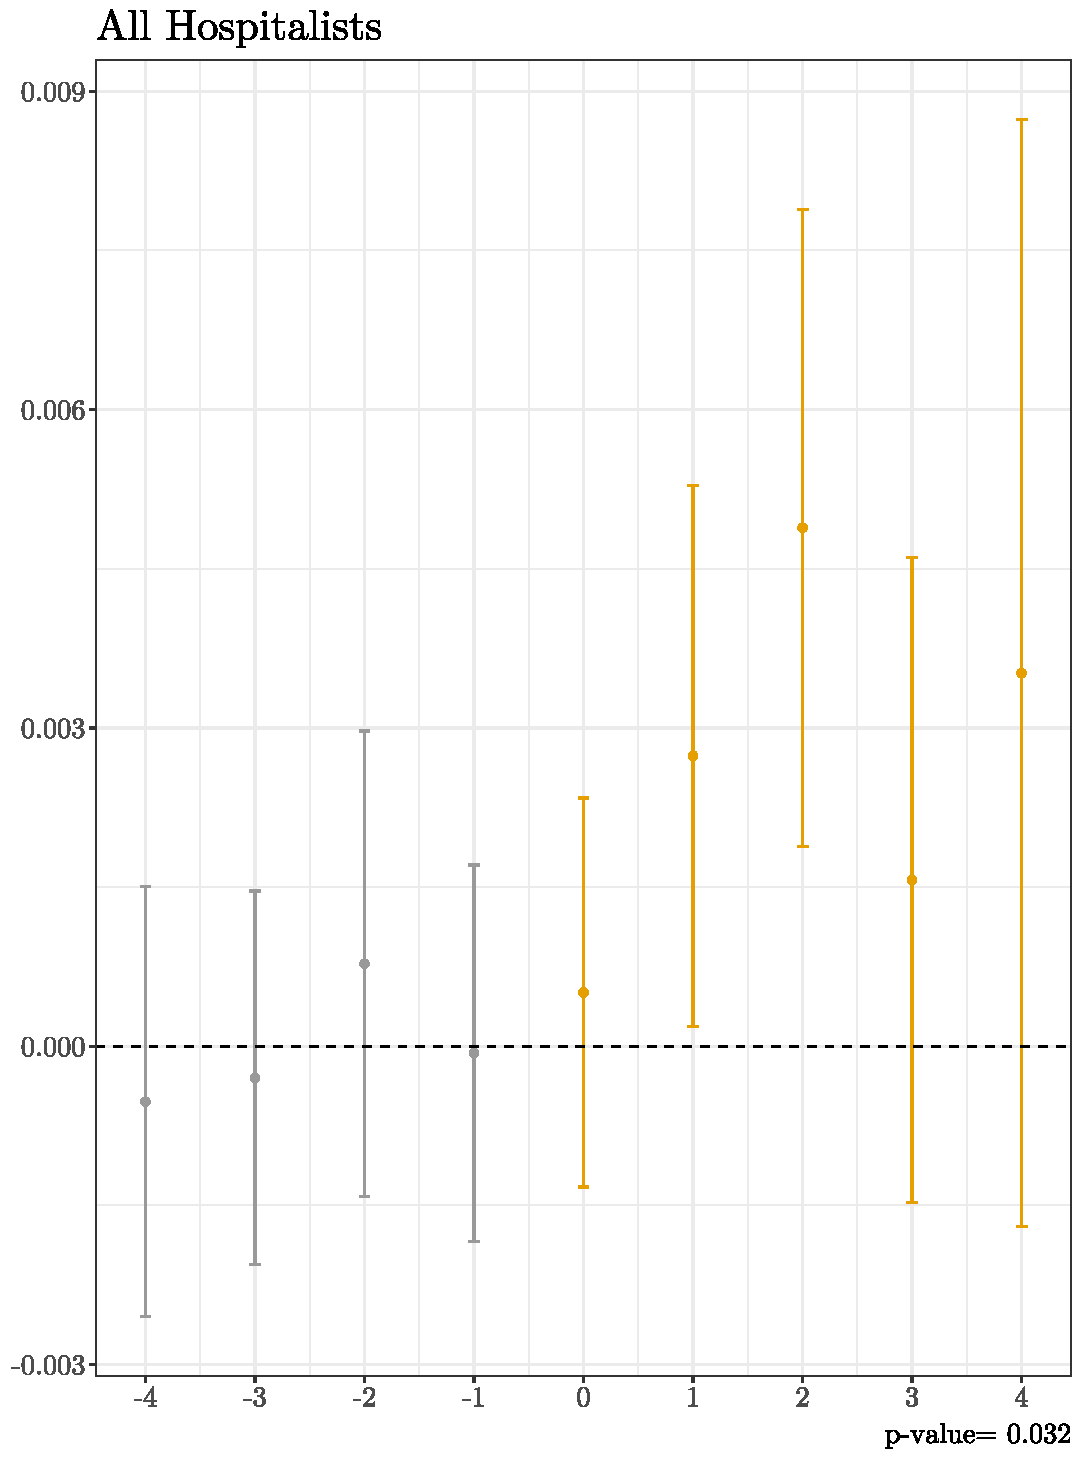
\includegraphics[scale=.4]{Objects/Presentation_retire_all.pdf}
\end{figure}
\end{frame}

\begin{frame}{Retirement: Senior Physicians}
\begin{figure}[ht]
    \centering
    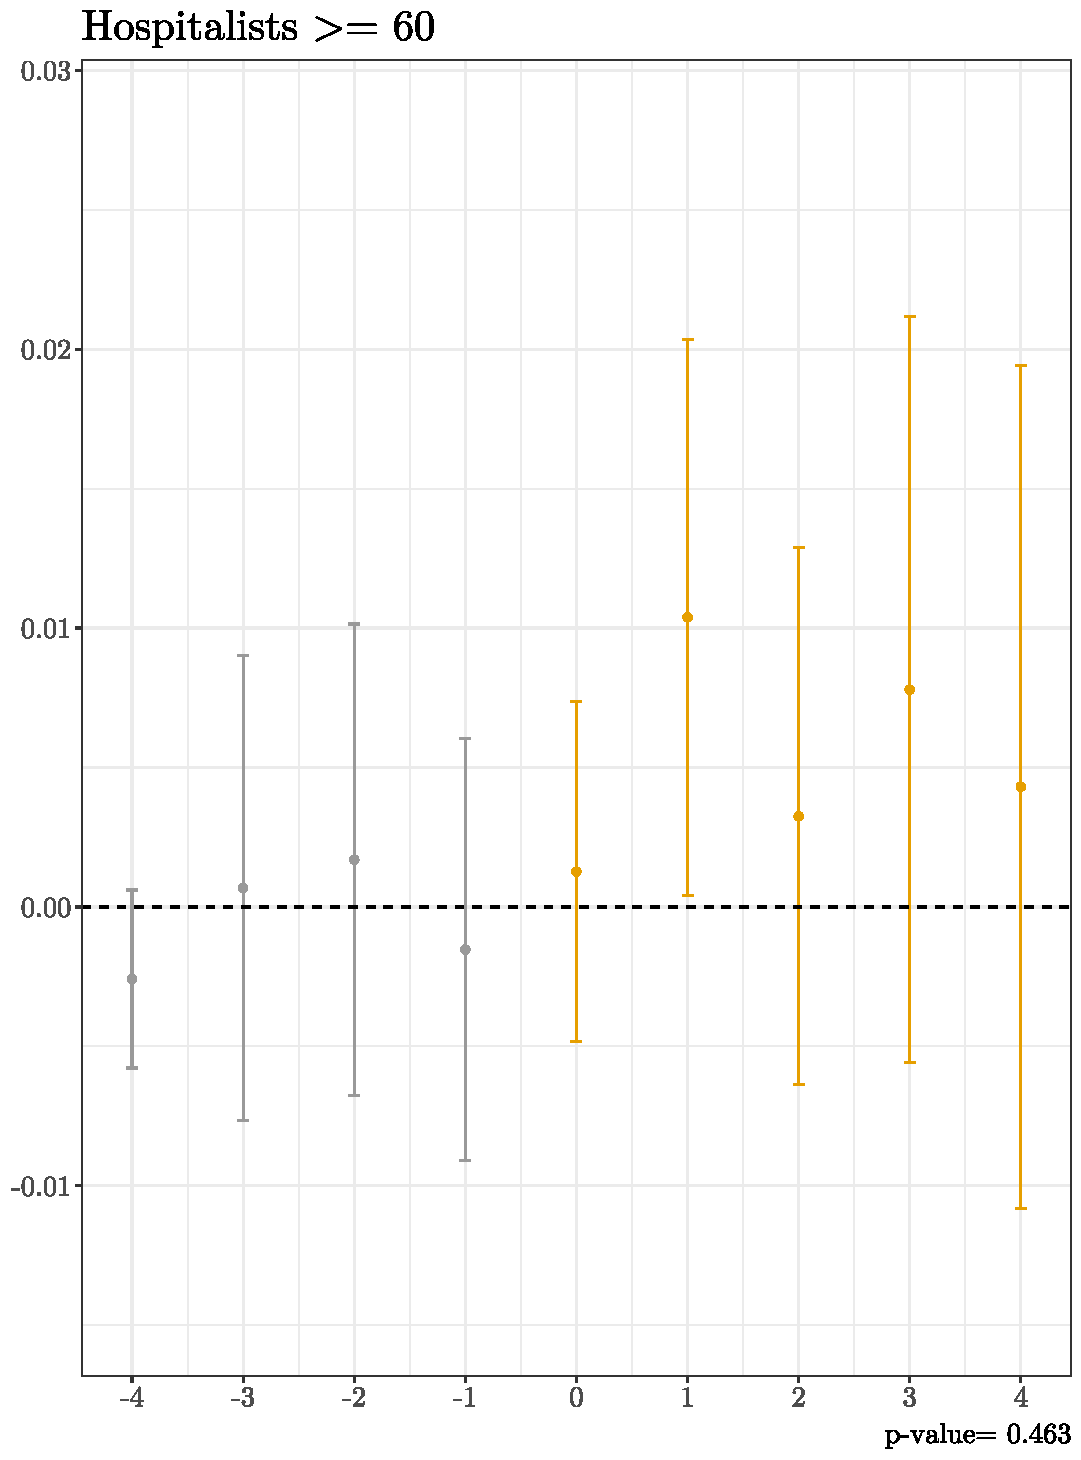
\includegraphics[scale=.4]{Objects/Presentation_retire_old.pdf}
\end{figure}
\end{frame}

\begin{frame}{Number of Patients Seen in Office}
\begin{figure}[ht]
    \centering
    \includegraphics[scale=.4]{}
\end{figure}
\end{frame}

\begin{frame}{Indicator for working in office}
\begin{figure}[ht]
    \centering
    \includegraphics[scale=.4]{}
\end{figure}
\end{frame}

\begin{frame}{Change Zip}
\begin{figure}[ht]
    \centering
    \includegraphics[scale=.4]{}
\end{figure}
\end{frame}

\begin{frame}{Patient Count}
\begin{figure}[ht]
    \centering
    \includegraphics[scale=.4]{}
\end{figure}
\end{frame}

\begin{frame}{Claims per Patient}
\begin{figure}[ht]
    \centering
    \includegraphics[scale=.4]{}
\end{figure}
\end{frame}

\begin{frame}{Summary}
\begin{itemize}
    \item Evidence that physicians are changing their behavior because of this new technology, specifically through retirement or job switching
    \item Little evidence of work setting changes
    \item For physicians who endure through the implementation of the technology, claims per patient goes down. 
    
\end{itemize}
\end{frame}







\section{Continuing Work}

\begin{frame}{Plans for this paper}
    \begin{itemize}
        \item Analysis on retirement decision of physicians: requires a better understanding of why physicians would drop out of this Medicare data
        \item See if there are any specific years driving these results
        \item Endogenous treatment? (Bandwidth, state privacy laws as IV)
    \end{itemize}
\end{frame}

\begin{frame}[plain]{}
\centering
    Thank you!
\end{frame}



\end{document}